\ifdefined\HANDOUT
\documentclass[handout]{beamer}
\else
\documentclass{beamer}
\fi

\mode<presentation>
{
  \usetheme{Warsaw}
  \definecolor{mcgarnet}{rgb}{0.38, 0, 0.08}
  \definecolor{mcgray}{rgb}{0.6, 0.6, 0.6}
  \setbeamercolor{structure}{fg=mcgarnet,bg=mcgray}
  %\setbeamercovered{transparent}
}


\usepackage[english]{babel}
\usepackage[latin1]{inputenc}
\usepackage{times}
\usepackage[T1]{fontenc}
\usepackage{tikz}
\usepackage{graphicx}

\newcommand{\imagesource}[1]{{\centering\hfill\break\hbox{\scriptsize Image Source:\thinspace{\small\itshape #1}}\par}}

\title{Data Preprocessing}


\author{Robert Lowe\\}

\institute[Maryville College] % (optional, but mostly needed)
{
  Division of Mathematics and Computer Science\\
  Maryville College
}

\date[]{}
\subject{}

\pgfdeclareimage[height=0.5cm]{university-logo}{images/Maryville-College}
\logo{\pgfuseimage{university-logo}}



\AtBeginSection[]
{
  \begin{frame}<beamer>{Outline}
    \tableofcontents[currentsection]
  \end{frame}
}


\begin{document}

\begin{frame}
  \titlepage
\end{frame}

\begin{frame}{Outline}
  \tableofcontents
\end{frame}


% Structuring a talk is a difficult task and the following structure
% may not be suitable. Here are some rules that apply for this
% solution: 

% - Exactly two or three sections (other than the summary).
% - At *most* three subsections per section.
% - Talk about 30s to 2min per frame. So there should be between about
%   15 and 30 frames, all told.

% - A conference audience is likely to know very little of what you
%   are going to talk about. So *simplify*!
% - In a 20min talk, getting the main ideas across is hard
%   enough. Leave out details, even if it means being less precise than
%   you think necessary.
% - If you omit details that are vital to the proof/implementation,
%   just say so once. Everybody will be happy with that.
\section{The Problem}
\begin{frame}{Database Field Issues}
\begin{itemize}[<+->]
   \item Data can be redundant.
   \item Data can be obsolete.
   \item The design decisions of the past haunt the future!
   \item Sensors are noisy.
   \item People are unpredictable, hence they make mistakes in data entry.
\end{itemize}
\end{frame}

\begin{frame}{Example Data Table}
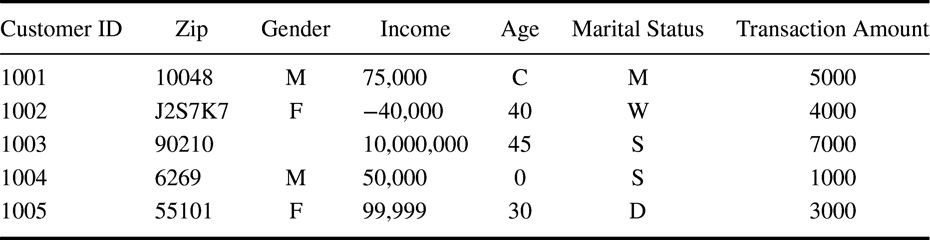
\includegraphics[width=\textwidth]{images/table-2-1}
{\tiny{\em Data Mining and Predictive Analytics} D. Larose p. 21}
\end{frame}

\begin{frame}{HAB Temperature Data - Raw}
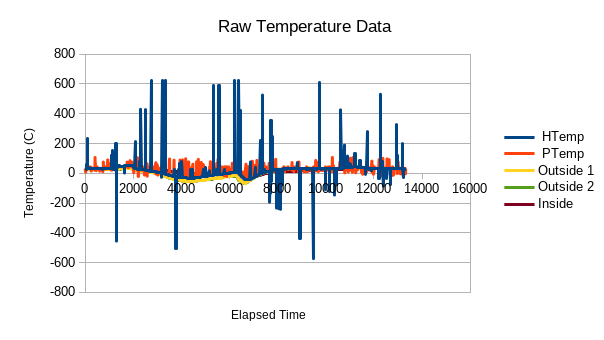
\includegraphics[width=\textwidth]{images/rawtemp}
{\tiny Collected October 7, 2017 over Athens, TN}
\end{frame}

\section{Data Cleaning}
\begin{frame}{Handling Missing Data}
We have options:
\begin{itemize}[<+->]
  \item Replace missing data with some constant value we select.
  \item Replace missing data with a field average.
  \item Replace missing data with a sentinel indicating that it is missing.
  \item Imputing new values.
\end{itemize}
\end{frame}

\begin{frame}{Handling Misclassification}
\begin{columns}
  \column{0.5\textwidth}
  \begin{itemize}[<+->]
  \item Sometimes categories are improperly split.
  \item Usually fixed by collapsing categories, reducing the separation.
  \item Watch for misspelled categories, but be careful!
  \end{itemize}
  
  \column{0.5\textwidth}
  \begin{tabular}{l|r}
  {\bf Category} & {\bf Count} \\
  \hline
  Sports & 25 \\
  News & 38 \\
  Footbal & 1\\
  \end{tabular}
\end{columns}
\end{frame}


\section{Data Transformation}
\begin{frame}{Overfitting and The Allure of Big Values}
\begin{itemize}[<+->]
  \item Large values can dominate data mining models.
  \item Some machine learning techniques will assign greater influence to large values.
  \item Proportional relationships within variables are often what we are after.
  \item We frequently apply some sort of normalization to variables.
\end{itemize}
\end{frame}

\begin{frame}{Center and Spread}
Recall the standard ways to describe a distribution: 
\begin{itemize}[<+->]
  \item Mean (center)
  \[
  \bar{X}=\displaystyle\frac{1}{n}\sum x_i
  \]
  \item Standard Deviation (spread)
  \[
  s = \sqrt{\displaystyle\frac{\sum (x_i-\bar{X})^2}{n-1}}
  \]
  \item Median (center)
  \item 5-number summary (distribution)
  \item Inter Quartile Range (Spread)
  \[
  IQR = Q_3 - Q_1
  \]
  \item Mode (center/typical value)
\end{itemize}
\end{frame}

\begin{frame}{Min-Max Normalization}
\[
X^*_{mm} = \displaystyle\frac{X - \mathrm{min}(X)}{\mathrm{max}(X) - \mathrm{min}(X)}
\]
\begin{itemize}[<+->]
\item Scales distance from min by the range.
\item All values are between 0 and 1.
\item Relative proportions of the values are left undisturbed.
\end{itemize}
\end{frame}

\begin{frame}{Z-Score Standardizaion}
\[
z = \displaystyle\frac{x-\bar{x}}{s}
\]
\begin{itemize}[<+->]
  \item Scales a variable to the number of standard deviations from the mean.
  \item Technically has infinite range, though for most data it ranges from -3 to 3.
\end{itemize}
\end{frame}

\begin{frame}{Decimal Scaling}
\[
X^*_{\mathrm{decimal}} = \displaystyle\frac{X}{10^d}
\]

\begin{itemize}[<+->]
  \item Where $d$ is the number of digits in the value with the largest absolute value.
  \item All values are between -1 and 1.
\end{itemize}
\end{frame}


\section{Variable Removal}
\begin{frame}{Variables to Remove}
  \begin{itemize}[<+->]
    \item Unary variables.
    \item Variables that are nearly unary.
    \item ID Fields (We should at least exclude them from our models!)
    \item Duplicate Records (With Care!)
  \end{itemize}
\end{frame}

\begin{frame}{Tempting Variables to Not Delete}
  \begin{itemize}[<+->]
  \item Variables with 90\% or more missing data.
  \item Variables that are strongly correlated.
  \item Records with missing values.
  \begin{block}{Missing Data in Records}
    If only 5\% of data values are missing
    from a data set of 30 variables, and the missing values are
    spread evenly throughout the data, almost 80% of the records would
    have at least one missing value."
    {\tiny \em --Gallit Shmueli, Nitin Patel, and Peter Bruce, Data Mining for
      Business Intelligence, 2nd edition, John Wiley and Sons, 2010. }
  \end{block}
    \end{itemize}
\end{frame}


\section{Homework}
\begin{frame}{Homework}
  \begin{itemize}
    \item P.52 13-23
    \item P.53 33-42 (Use R and make a printed writeup)
  \end{itemize}
\end{frame}
\end{document}


